\documentclass[letterpaper]{article}
\usepackage[spanish,es-tabla]{babel}
\usepackage{indentfirst}
\usepackage{float}
\usepackage[utf8]{inputenc}
\usepackage{graphicx}

\begin{document}
    
\subsection{Implementación fftshift}
Los resultados que se obtienen al utilizar la \textit{fftshift} son:
\begin{figure}[]
    \centering
    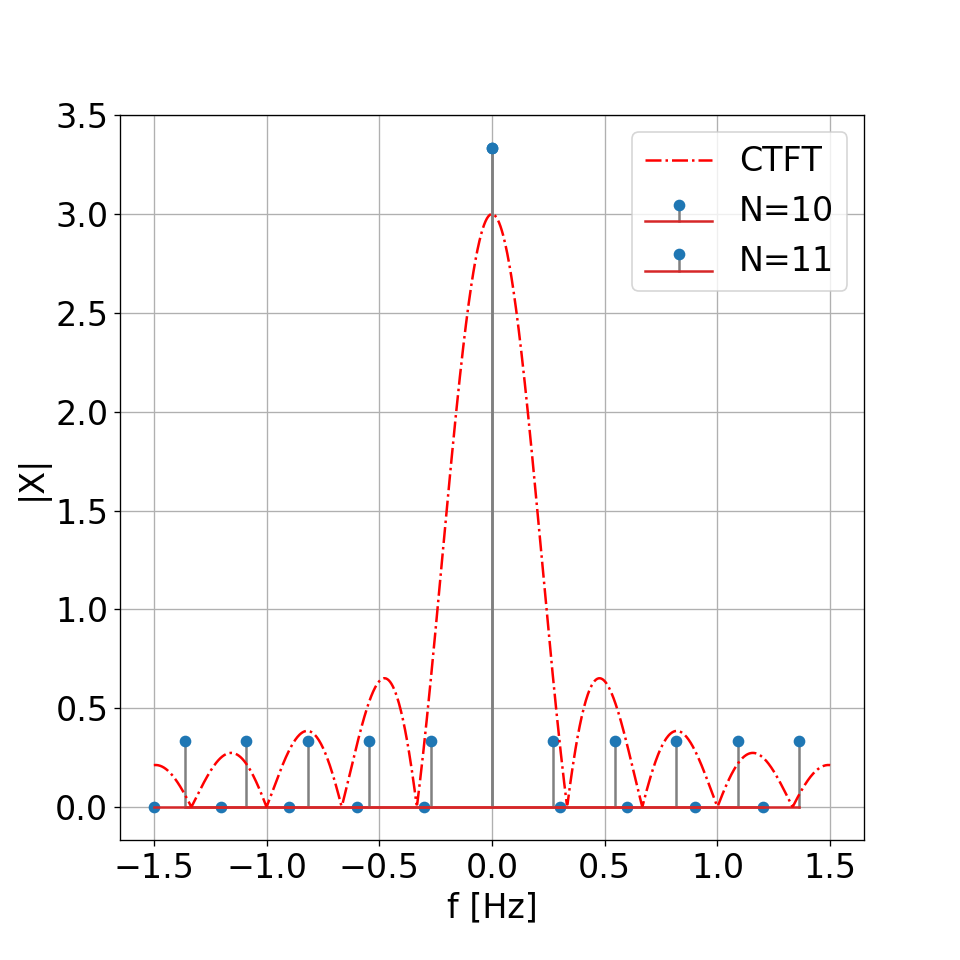
\includegraphics[width=\textwidth]{Img/punto_4_f.png}
    \caption{}
    \label{fftshift}
\end{figure}
En la figura \ref{fftshift} se aprecia que al utilizar la \textit{fftshift} las muestras de la fft no coinciden con el espectro deseado de la CTFT. Sin embargo,
estas muestras son representaciones exactas de la DTFT de la señal muestreada. Esta disparidad se debe al aliasing presente en la forma de implementación de la DFT.\\
Para utilizar de forma correcta la \textit{fftshift} se deben cumplir las condiciones propuestas en el \ref{inciso c)}. Esto permite obtener una visualización que se aproxime de mejor 
forma al espectro de la CTFT. 


\end{document}